\documentclass[11pt]{article}
\usepackage[sc]{mathpazo} %Like Palatino with extensive math support
\usepackage{fullpage}
\usepackage[authoryear,sectionbib,sort]{natbib}
\linespread{1.7}
\usepackage[utf8]{inputenc}
\usepackage{lineno}

%%%%%%%%%%%%%%%%%%%%%
% LaTeX packages
%%%%%%%%%%%%%%%%%%%%%
% Please be sparing in your use of additional LaTeX packages, and
% upload any required style files to Editorial Manager with the file
% type "LaTeX ancillary files (.sty, .bst)."
\usepackage{amsmath}
\usepackage{graphicx} %remove when remove figures
\graphicspath{ {IMAGES/} }

%%%%%%%%%%%%%%%%%%%%%
% Line numbering
%%%%%%%%%%%%%%%%%%%%%
\usepackage{lineno}
% Please use line numbering with your initial submission and
% subsequent revisions. After acceptance, please comment out 
% the commands \usepackage{lineno}, \linenumbers{} 
% and \modulolinenumbers[3] below.

\title{The temperature-size rule is predicted to stabilize consumer-resource dynamics under warming\\
or\\
Temperature-dependent body size alters the effects of temperature on consumer resource dynamics}

%%%%%%%%%%%%%%%%%%%%%
% Authorship
%%%%%%%%%%%%%%%%%%%%%
% Please remove authorship information while your paper is under review,
% unless you wish to waive your anonymity under double-blind review. 
% Remember to uncomment the information after acceptance.

%\author{Matthew Miles Osmond$^{1,\ast}$ \\ 
%et al$^{2}$}

\date{}

\begin{document}

\maketitle

%\noindent{}1. Biodiversity Research Centre and Department of Zoology, University of British Columbia, Canada;
%
%\noindent{}2. others;
%
%\noindent{}$\ast$ Corresponding author; e-mail: mmosmond@zoology.ubc.ca.

\bigskip

\textit{Manuscript elements}: Figure~1, figure~2, figure~3, supplementary \texttt{Mathematica} file.
\bigskip

\textit{Keywords}: Metabolic theory, predator-prey, plant-herbivore, body size, allometry, functional response, mathematical model.

\bigskip

\textit{Manuscript type}: Note. 
% Or e-article, note, e-note, natural history miscellany,
% e-natural history miscellany, comment, reply, symposium, or
% countdown to 150.

\bigskip

\noindent{\footnotesize Prepared using the suggested \LaTeX{} 
template for \textit{Am.\ Nat.}}

\linenumbers{}
\modulolinenumbers[3]

\newpage{}

%%%%%%%%%%%%%%%%%%%%%%%%%%%%%%%%%%%%%%%%%%%%%%%%
\section*{Abstract}
%%%%%%%%%%%%%%%%%%%%%%%%%%%%%%%%%%%%%%%%%%%%%%%%
Both body size and temperature directly influence the dynamical relationship between consumers and their resources. There is also a widespread negative relationship between temperature and size; this is known as the temperature-size rule (TSR). The growing theory on temperature-dependent consumer resource interactions has yet to integrate the TSR into a general framework for how temperature affects consumer resource dynamics. 
We expanded an existing temperature-dependent consumer-resource model to include the indirect effects of warming, through changes in body size, and parameterized the model with values drawn from data syntheses. 
We analyzed this model to answer the following questions: 
1) How does including the TSR affect predictions for how temperature affects consumer-resource stability and biomass ratios? 
2) Under what circumstances are the effects of the TSR most substantial? 
%3) Is the TSR predicted to induce a change in the functional response? 
We found that including the TSR led to two qualitatively different predictions: under warming i) consumer-resource biomass is no longer expected to decline and ii) the dynamics are expected to become more stable, as opposed to the decline in stability predicted without the TSR. 
These qualitatively different predictions were strengthened by asymmetric temperature-size responses between consumers and resources and type-II functional responses.
Our analyses suggest that the effect of temperature on body size likely plays an important role in the response of consumer-resource systems to changing temperatures. 

\newpage{}

%%%%%%%%%%%%%%%%%%%%%%%%%%%%%%%%%%%%%%%%%%%%%%%%
\section*{Introduction}
%%%%%%%%%%%%%%%%%%%%%%%%%%%%%%%%%%%%%%%%%%%%%%%%

% The journal does not have numbered sections in the main portion of
% articles. Please refrain from using section references such as
% section~\ref{section:CountingOwlEggs}, and refer to sections by name
% (e.g. section ``Counting Owl Eggs'').

% Please note that we prefer (\citealt{Xiao2015}) to \citealt{Xiao2015},
% since \citealt{} inserts a comma after "et al."

%%%%%%%%%%%%%%%%%%%%%%%%%%%%%
%my little weekend attempt

%Temperature and body size determine many biological rates (\cite{West1997,Gillooly2001}).
%How these factors individually influence consumer-resource dynamics has already been demonstrated (\cite{Gilbert2014,DeLong2015}).
%How they act in symphony has not yet been investigated.
%
%Temperature also affects body size through the temperature-size rule (\cite{Atkinson1994}).
%Thus, temperature directly and indirectly affects ecosystem dynamics.
%These two pathways have the potential to reinforce or counteract one another, with population level consequences.
%
%Here we model a simple consumer-resource interaction, with population dynamic parameters that depend on temperature and body size, and body sizes that depend on temperature.
%We ask how including dependencies on both temperature and body size, as well as incorporating the temperature-size rule, affects the response of the consumer-resource dynamics to increasing temperature.

%%%%%%%%%%%%%%%%%%%%%%%%%%%%%

Populations of consumers and their resources are joined across time by the flow of energy from resource to consumer, and the mortality imposed on the resource by this flow. 
In such a system, temperature-dependent consumption, growth, and mortality can change dynamics and their outcomes. 
Through the temperature-dependence of metabolism \citep{West1997,Gillooly2001} demographic vital rates change with temperature.
Small changes in temperature that are not necessarily physiologically stressful for organisms can thus translate to changes in the stability and coexistence of consumers and their resources,  producing predictable effects of warming on simple food webs \citep{Gilbert2014,Vasseur2005,OConnor2011,Rall2010}. 

Demographic rates in consumer-resource systems also depend on the body sizes of the interacting agents\citep{Yodzis1992,DeLong2015}. 
In addition, the rate at which the consumer consumes the resource can depend on their body size ratio \citep{Kalinkat2013}. 
Changes in body size or body size ratios therefore change demographic and interaction rates. 
Given the importance of body size to the dynamics and outcomes of consumer-resource interactions, frameworks for understanding how temperature affects consumer-resource dynamics should consider the importance of changes in body size with temperature, but they currently do not.

The frequently-observed negative relationship between temperature and body size, the temperature-size rule (TSR), is considered a universal response to warming \citep{Gardner2011}. 
% * <mwpennell@gmail.com> 2016-06-24T21:49:24.120Z:
%
% pedantic point: does the TSR describe a response to changes in temperature or simply a negative relationship between the two
%
% ^ <mwpennell@gmail.com> 2016-06-24T21:51:49.434Z:
%
% and also: what are the other two? seems odd to mention this as the third without that context
%
% ^.
For comparisons within populations, among species, and across biogeographic gradients, body size of ectotherms tends to decline with increasing temperature \citep{Atkinson1994,Daufresne2009,Forster2012,DeLong2012}. 
Although the mechanism for declining body size with warming varies among examples (e.g., physiological plasticity, selection for smaller individuals, and turnover in species composition) the pattern is similar across levels of organization \citep{Forster2012}. 
In a comprehensive meta-analysis involving 169 species, \citet{Forster2012} reported a mean body mass decline of -3.65$\%$ per $^\circ C$ for aquatic organisms, ranging from -1.80$\% / ^\circ C$ in unicellular taxa and becoming stronger (more negative) in increasingly large aquatic multicellular species.

Because body size is central to consumer-resource dynamics \citep{Yodzis1992}, such a systematic pattern of changing body size with temperature could alter predictions for how temperature affects stability, persistence, and coexistence in consumer-resource systems. 
We therefore integrated the TSR into a general framework for temperature-dependent consumer-resource interactions to answer the following questions: 
1) How does the TSR affect consumer:resource biomass ratios and stability over a temperature gradient?, 
2) How does the effect of the TSR depend on how strongly and similarly consumer and resource body sizes respond to temperature?, 
3) Does the effect of the TSR depend on the form of the functional response?, 
And finally, 4) does the TSR itself induce a change in the functional response?

%%%%%%%%%%%%%%%%%%%%%%%%%%%%%%%%%%%%%%%%%%%%%%%%%%%
\section*{Methods and results}
%%%%%%%%%%%%%%%%%%%%%%%%%%%%%%%%%%%%%%%%%%%%%%%%%%%

%%%%%%%%%%%%%%%%%%%%%%%%%%%
\subsection*{The underlying consumer-resource dynamics}
%As an aside, I've always found it interesting that the Rosenzweig-MacArthur equations are attributed to this paper, although I've never been able to clearly identify these equations in the paper.\
%yeah, it looks like you could translate their equation 1 and 2a into these equations if you wished, but good observation! (MMO)
We begin, like \cite{Gilbert2014}, with the Rosenzweig-MacArthur equations \citep{Rosenzweig1963}
\begin{equation}\label{eq:RM}
\begin{aligned}
\frac{\mathrm{d}R}{\mathrm{d}t} =& r R \left(1 - \frac{R}{K} \right) - f(R) R C\\
\frac{\mathrm{d}C}{\mathrm{d}t} =& e f(R) R C - m C,
\end{aligned}
\end{equation}
which describe the rates of change in total resource $R\in[0,K]$ and consumer $C\geq0$ biomass with time $t$.

In the absence of consumers, $C=0$, the resource grows logistically, with intrinsic growth rate $r\geq0$ and carrying capacity $K>0$.
The intrinsic growth rate describes the rate at which resource biomass increases (per unit biomass) in the absence of consumers when the resource is rare, $R\approx0$.
The carrying capacity is the equilibrium biomass of the resource without consumers.

Resource biomass is consumed by consumers at a rate $f(R) R C$, where $f(R)\geq0$ is called the functional response.
Of the biomass consumed, the unitless conversion efficiency parameter $e\in[0,1]$ determines the proportion of resource biomass that is directly converted into consumer biomass.
Consumers biomass dies at a constant per unit biomass mortality rate $m\geq0$.

An equilibrium is reached when the two rates of change in Equation \eqref{eq:RM} are zero, and solving the system at this point gives equilibrium resource $\hat{R}$ and consumer $\hat{C}$ biomass.
There are three equilibria for this system: total extinction $(R,C) = (0,0)$, consumer extinction $(R,C)=(K,0)$, and coexistence $(R,C)=(\hat{R},\hat{C})$, with $\hat{R}>0$ and $\hat{C}>0$.
We are primarily concerned with the latter equilibrium, as this is presumably the equilibrium current consumer-resource systems are near. %(we would not consider them consumer-resource systems if either the consumer or resource were absent).
At this coexistence equilibrium one can calculate the ratio of consumer to resource biomass, $\hat{C}:\hat{R}$, and also perform a linear stability analysis to derive the leading (largest in absolute value) eigenvalue $\lambda$, which determines if (and how readily) the system, when perturbed a small amount from this equilibrium, will return to it (see supplementary \texttt{Mathematica} file for details).
Our measure of stability will be the negative of the real part of the leading eigenvalue.
%I think I'm getting confused by the wording here in lines 170 and 171. For a continuous time model such as this one, doesn't a negative eigenvalue correspond to a stable system?
%yeah, thats right. Gilbert just took the negative of this (giving a positive) to describe "how stable" something is. (MMO)
The system is stable if and only if this value is positive, and the system will return to equilibrium faster when this value is larger (i.e., larger positive values imply ``more stable" systems).
Together these two measures tell us how biomass is partitioned and how stable this partitioning is.

As explained in \cite{Gilbert2014}, two aggregate parameters well describe the dynamics of this system.
The first is $m /(e f(\hat{R}))$, which i) describes (the inverse of) consumer growth at equilibrium, ii) is the slope of the consumer zero-net growth isocline, and iii) is the abundance of the resource at the coexistence equilibrium.
The second aggregate is $K$, the equilibrium resource biomass in the absence of consumers.
Dividing the second aggregate by the first gives a measure that defines the biomass potential of the resource that is converted into consumer biomass \[B_{CR} = \frac{e f(\hat{R}) K}{m}.\]
%Note that we have modified the presentation of \cite{Gilbert2014} by subsuming $R$ into $f(R)$ such that $f(R)$ is  a rate and thus more easily interpreted.
%This does not alter the results.

In what follows we will examine how our three measures, $B_{CR}$, $\hat{C}:\hat{R}$, and stability, change with temperature.
We start by assuming a type-I functional response, $f(R) = a$, where $a$ is called the attack rate, which describes the rate of resource consumption per resource biomass.
We later explore the effect of a type-II functional response and the potential for the functional response to change with changes in temperature.

%%%%%%%%%%%%%%%%%%%%%%%%%%%
\subsection*{Adding temperature dependence}

\cite{Gilbert2014} discuss what is known about the temperature dependencies of the population dynamic parameters $r$, $K$, $a$, $m$, and $e$, and give equations and parameter estimates (from previously published sources) in their Table 1.
Briefly, resource growth rate $r$ is expected to scale with metabolism as a Boltzmann-Arrhenius factor, 
\[r(T) = r_0 \exp \left(-\frac{E_B}{kT} \right),\] 
where $E_B$ is the activation energy of metabolism $B$ (in units of eV), $k$ is Boltzmann's constant ($\approx 8.62 \times 10^{-5}$ eV/Kelvin), and $T$ is the temperature (in Kelvins).
Resource carrying capacity $K$ is determined by the ratio of the supply rate of nutrients into the system, S, and the rate of uptake of nutrients by the resource, $r$.
With supply rate also scaling as a Boltzmann-Arrhenius factor with activation energy $E_S$, the prediction for carrying capacity becomes
\[K(T) = K_0 \exp \left(-\frac{E_S - E_B}{kT} \right).\] 
Attack rate $a$ depends on the temperature dependence of the body velocities $\nu$ in both species, both of which scale as Boltzmann-Arrhenius factors with activation energies $E_{\nu,i}$, for $i=\{R,C\}$.
Attack rate is then 
\[a(T) = a_0 \sqrt{\sum_i \left[\nu_{0,i} \exp \left(-\frac{E_{\nu,i}}{kT} \right) \right]^2},\] 
where $\nu_{0,i}$ are rate-constants.
Consumer mortality is also expected to scale as a Boltzmann-Arrhenius factor, 
\[m(T) = m_0 \exp \left( -\frac{E_m}{kT} \right).\]
Conversion efficiency is assumed to be independent of temperature such that $e(T) = e_0$.

The black curves in Figure \ref{AllTempMassDep} show $B_{CR}$, equilibrium consumer to resource biomass ratio $\hat{C}:\hat{R}$, and stability of the coexistence equilibrium as functions of temperature $T$ (plotted in Celsius). This is comparable to Figure 3 of \citet{Gilbert2014}, except that in their version of the figure, only $K$ depends on temperature; everything else is held constant. If we consider all of the additional dependencies discussed by \citet{Gilbert2014}, we see that adding temperature dependence in $r$, $a$, and $m$ causes $\hat{C}:\hat{R}$ to decline with temperature (instead of increasing) and stability to decrease at a slower rate with increasing temperature.
These changes are largely driven by the temperature dependence of consumer mortality: increasing temperature increases consumer mortality, lowering equilibrium consumer biomass and increasing stability at high temperatures (relative to the case where mortality $m$ does not depend on temperature; see supplementary \texttt{Mathematica} file for details).
% * <barbour@zoology.ubc.ca> 2016-06-24T13:58:58.890Z:
%
% MO: why do you attribute the decline in C:R biomass and relatively greater stability to higher consumer mortality (primarily)? Is the logic something like: increasing m, by itself, would create this pattern; increasing r, by itself, would increase C:R, but also increase stability (at least in type 1); and increasing a, by itself, would increase C:R, but decrease stability? I'm mainly asking to also check my understanding of the influence of different parameters on C-R models.
%
% ^.
%no, this isn't a logic thing at all but simply me including or excluding the temperature dependence of parameters in the mathematica file until i find which one is driving the pattern. so here for example, when i make m temperature-independent the prediction looks much like gilberts, and dropping temp dependence of the other parameters does not affect things as much. (MMO)

%%%%%%%%%%%%%%%%%%%%%%%%%%%
\subsection*{Adding mass dependence and the temperature size-rule}

We next allow the population dynamic parameters to depend on the body size of the interacting species.
Following \cite{DeLong2015}, each parameter can be written as a power law function of the body mass of resource $M_R$ or consumer $M_C$.
Here we combine \cite{DeLong2015} and \cite{Gilbert2014} by letting the parameters depend on both temperature and mass: $r(T, M_R) = r(T) M_R^\rho$, $K(T, M_R) = K(T) M_R^\kappa$, $a(T, M_C) = a(T) M_C^\alpha$, $e(T, M_C) = e(T) M_C^\epsilon$, and $m(T, M_C) = m(T) M_C^\mu$.

If mass does not change with temperature then adding these mass dependencies does not change the response of the consumer-resource dynamics to temperature.
However, mass is expected to change with temperature, according to the temperature-size rule \citep{Atkinson1994}.
%For organisms with a dry mass of less than $10^{-3}$ mg body mass declines linearly with temperature.
We incorporate a simple form of the temperature-size rule here for illustrative purposes.
In particular, we assume body mass declines linearly with temperature, 
\[M_i(T) = M_i(T_{ref}) [1 - \beta_i (T - T_{ref})], \]
where, $i=\{R,C\}$, $\beta_i$ is the fraction that mass is reduced as temperature is increased by one degree, and $T_{ref}$ is a reference temperature, which we set to 15$^\circ C$ throughout.
This linear decline best approximates the response of organisms with a dry mass of less than $10^{-3}$ mg, whereas larger organisms experience a faster than linear decline \citep{Forster2012}.

The red curves in Figure \ref{AllTempMassDep} depict our main results: adding mass dependencies and the temperature-size rule modifies our prediction of how consumer-resource dynamics respond to changes in temperature.
While there is little change in $B_{CR}$, the equilibrium consumer to resource biomass ratio $\hat{C}:\hat{R}$ is no longer expected to decline with increasing temperature and stability is now expected to increase.
These changes are brought on by the indirect effect of temperature, through body mass, on the population dynamic parameters, which are acting in opposition to its direct effects.
In particular, the lack of decline in $\hat{C}:\hat{R}$ with the temperature-size rule, relative to the case without it, is primarily driven by changes in consumer conversion efficiency and the intrinsic growth rate of the resource (see supplementary \texttt{Mathematica} file).
Both of these rates increase with declining body mass, supporting a relatively larger consumer biomass. 
The increase in stability at high temperatures with the temperature-size rule is caused by the increase in the resource's intrinsic growth rate along with a decrease in attack rate with decreasing consumer body size. 
% * <barbour@zoology.ubc.ca> 2016-06-24T13:58:32.133Z:
%
% It looks like mortality rate would also increase with declining body mass, won't this also contribute to increased stability (although I understand that it would decrease C:R)
%
% ^.
%logic is like that explained above: i just drop the mass dependencies of each parameter in turn and see which ones are having the largest effect (see mathematica file) (MMO)
%
%The indirect effects of temperature are acting in opposition to its direct effects.
So we see that in the case of stability, the indirect effect of temperature, through body mass, is strong enough to override its direct effect on demographic parameters, producing a qualitatively different prediction of how consumer-resource systems will respond to temperature.
%The increase in stability with the temperature-size rule stimulates the tantalizing possibility that its existence is adaptive, although obviously much more careful thought is needed here.

In the supplementary \texttt{Mathematica} file we explore how the strength of the temperature-size response $\beta_C = \beta_R = \beta$ affects our predictions (see also Figure \ref{StrengthAsymm}, green). 
We find that predictions for biomass ratio and stability at higher temperatures differ qualitatively from those of \cite{Gilbert2014} for $\beta\geq0.02$.
The equilibrium biomass ratio begins to increase with temperature around $\beta\sim0.03$.
Larger temperature-size responses cause faster increases of biomass ratio and stability with temperature. %(and decrease faster with declining temperature).

%%%%%%%%%%%%%%%%%%%%%%%%%%%
\subsection*{Exploring asymmetric temperature-size responses}

In Figure \ref{AllTempMassDep} we assumed both resource and consumer body mass declined proportionally with temperature at the same rate, $\beta_C = \beta_R$. %= 0.02$, i.e., both decline $2\%$ per degree increase.
However, larger organisms often experience larger proportional declines in body size with temperature (\cite{Forster2012}).
%In Figure \ref{AllTempMassDepAsymm} we let consumer body size decline twice as fast as the resource, $2 \beta_R = \beta_C = 0.04$.
To explore this effect, in Figure \ref{StrengthAsymm} (blue) we let consumer body size decline twice as fast as the resource, $2 \beta_R = \beta_C$.
The main effect of the asymmetric temperature-size response is that i) the $B_{CR}$ now asymptotes at higher temperatures (compare blue with red in Figure \ref{AllTempMassDep}A) and ii) stability now increases even faster with increasing temperature (compare blue with red in Figure \ref{AllTempMassDep}C).
These effects are driven by the now larger decline in attack rate.
Thus, expected asymmetries in the temperature-size response cause our predictions to deviate even further from those of without the temperature-size rule \citep{Gilbert2014}.

%%%%%%%%%%%%%%%%%%%%%%%%%%%
\subsection*{Type-II functional response}

The consumption of resources in some systems may be better described by a type-II functional response, 
\[f(R) = b / (1 + b h R),\] 
where $b$ is sometimes called the capture rate (the per resource biomass per consumer biomass rate of resource biomass consumption) and $h$ the handling time.
This collapses to a type-I functional response at low resource biomass, $f(R) \approx b$ for $R << 1/(b h)$.
At high resource biomass a type-II functional response implies that the rate of resource consumption per consumer biomass asymptotes at $\lim_{R\rightarrow\infty}f(R) R = 1/h$, describing satiation of the consumer.

Both capture rate and handling time are known to depend on temperature and body mass.
In particular, \cite{Rall2012} argue that capture rate scales like 
\[b(T, M_R, M_C) = b_0 M_R^{b_R} M_C^{b_C} \exp \left(- \frac{E_b}{k T} \right)\]
and handling time like 
\[h(T, M_R, M_C) = h_0 M_R^{h_R} M_C^{h_C} \exp \left(-\frac{E_h}{k T} \right).\]
With these scaling the type-II functional response increases faster with temperature than the type-I functional response (see supplementary \texttt{Mathematica} file) %shows how the functional response changes with temperature.
Much of the difference in the response of the functional responses to temperature is due to the differing temperature- and mass- dependencies of attack rate $a$ and capture rate $b$, and is not due to the form of the functional responses (i.e., setting $h=0$ has little effect on the response of the type-II functional response to temperature).
When capture rate has the same temperature- and mass- dependencies as attack rate (\cite{Gilbert2014}), there is little difference between the response of the type-I and type-II functional responses to temperature (see supplementary \texttt{Mathematica} file for details).

With the parameter values given in \cite{Rall2012}, we can plot $B_{CR}$, $\hat{C}:\hat{R}$, and stability as functions of temperature when there is a type-II functional response (Figure \ref{TypeII}).
The main conclusions are: in comparison to a type-I functional response, a type-II functional response i) makes $B_{CR}$ increase faster with temperature, ii) makes the equilibrium biomass ratio increase with temperature over the entire temperature range (instead of asymptoting), and iii) makes stability increase more quickly with temperature, despite the fact that a type-II functional response decreases stability at our reference temperature (15$^\circ$C, i.e., without a direct or indirect temperature response).
Thus, a type-II functional response, like asymmetric temperature-size responses, causes our predictions to vary further from those made without the temperature-size rule \citep{Gilbert2014}.
% * <barbour@zoology.ubc.ca> 2016-06-24T13:57:51.700Z:
%
% MO: just to clarify, was your exploration of the type 2 functional response always restricted to cases where the equilibrium was stable? I ask, because according to McCann (2012, book), increasing intrinsic growth rate has qualitatively different effects on stability depending on whether the consumer isocline is to the left or right of the resource's hump-shaped isocline. In other words, if the system is exhibiting a stable limit cycle, then increasing intrinsic growth rate will actually further destabilize the system.
%
% ^.
% yes, always where stable (i chose handling time such that this was true)

As an aside, in this analysis we choose $b_0$ to give $f(R) = 0.1$ at 15$^\circ C$, to remain consistent with \cite{Gilbert2014}.
This leaves $h_0$ as a free parameter. 
However, this free parameter influences stability.
When $h_0$ is small enough to allow a stable coexistence equilibrium (roughly $h_0 <10^{-12}$) we find that stability increases exponentially with temperature (blue curve in Figure \ref{TypeII}).
Thus, even though a type-II functional response decreases stability at the reference temperature (because of the lags induced by handling time), stability is increased at higher temperatures. 
The increased stability at higher temperatures with a type-II functional response is caused by the temperature dependence of the capture rate \citep{Rall2012}, which differs from the temperature dependence of the type-I attack rate \citep{Gilbert2014}.
Giving capture rate the same temperature dependence as attack rate \citep{Gilbert2014}, with a small enough handling time at the reference temperature ($h_0 <\sim10^{-13}$) stability still increases exponentially with temperature, but the square root in the expression now allows the temperature dependence of other parameters to slow and revert this increase at higher temperatures.
Larger handling times prevent the exponential increase in stability with temperature, and the increase in handling time with temperature can even cause stability to decrease with temperature (see supplementary \texttt{Mathematica} file for details). 

\cite{Rall2012} complied a large database on capture rates and handling times and compared the data to their theoretical predictions.
They found that capture rate and handling time responded less strongly to temperature than expected (see their Figure 2a,d).
Interestingly, we find that the temperature-size rule reduces the sensitivity of both capture rate and handling time to temperature (see supplementary \texttt{Mathematica} file) and hence may help explain the discrepancies observed. 

%%%%%%%%%%%%%%%%%%%%%%%%%%%
\subsection*{A functional response that depends on the body size ratio}

Functional responses tend to be more type-II when consumers and resources have similar body sizes, but become more sigmoidal and hence more type-III when consumers are much bigger than their resource, as resources are then better able to hide when rare \citep{Kalinkat2013}.
Without the temperature-size rule, the body mass ratio remains constant with temperature, and therefore the form of the functional response is not expect to change.
However, with the temperature-size rule, body sizes change.
When the temperature-size responses are asymmetric, the ratio of body sizes will change and influence the form of the functional response.
Because consumers are often larger than their resource, and because larger organisms are expected to have greater reductions in body size with temperature \citep{Forster2012}, the ratio of consumer to resource body size will often decrease with temperature.
As stated above, lower consumer to resource body size ratios produce functional responses more type-II, which are less stable than type-III functional responses.
Hence the temperature-size rule can be said to destabilize the consumer-resource dynamics at high temperatures by promoting type-II functional responses. %(it can also be said that the temperature-size rule stabilizes the dynamics at lower temperatures by promoting type-III functional responses).
However, the amount by which the shape of the functional response is adjusted by the temperature-size rule does not appear to be large and therefore the stabilizing effects discussed in previous sections will likely prevail (see supplementary \texttt{Mathematica} file for details). 

%%%%%%%%%%%%%%%%%%%%%%%%%%%%%%%%%%%%%%%%%%%%%%%%%%
\section*{Discussion}
%%%%%%%%%%%%%%%%%%%%%%%%%%%%%%%%%%%%%%%%%%%%%%%%%%%

%BIG PICTURE AND SUMMARY OF MAIN RESULTS
Our results suggest changes in body size with warming have important dynamical consequences for food webs in changing thermal environments. 
In our temperature- and mass-dependent consumer-resource model, declining body size with warming changes the predicted outcome of consumer-resource dynamics in response to temperature. 
When body sizes decline with warming at rates consistent with empirical observations \citep{Forster2012}, consumer-resource biomass ratios remain stable or increase under warming, compared to expected declines without the TSR. 
Furthermore, the TSR facilitates an increase in system stability with warming, relative to a decrease in stability without it. 
%At the same time, the bioenergetic interaction strength metric (BCR) is relatively unaffected by the TSR. 

%DIRECT VS INDIRECT
%When consumer and resource body sizes decline (proportionally) at the same rate with warming, there is no shift in the consumer to resource body size ratio over the temperature gradient. 
%In this case, deviations in how consumer and resource biomass respond to temperature, compared with a system with no TSR, reflects the body mass-dependence of demographic parameters. 
Deviations in the expected response of consumer-resource dynamics to temperature with a TSR, compared to a system without it, reflect the body mass-dependence of demographic parameters. 
In this way, temperature acts on the system both by directly altering demographic rates and by indirectly altering demographic rates through allometric scaling relationships. 
For instance, the resources's intrinsic growth rate is expected to be greater when the resource is smaller, and hence the indirect effect of warming allows the resource to support a relatively greater consumer biomass at higher temperatures. 
In this case the indirect and direct effects act in the same direction, and hence the indirect effect amplifies the response to temperature.
For other parameters, like attack rate, the indirect and direct effects oppose one another, and the indirect effect acts to dampen the response to temperature.

%STRENGTHS AND ASYMMETRIES
Although there are a number of theoretical explanations for the TSR \citep{Berrigan1994,Perrin1995,VanderHave1996,Angilletta2003,DeLong2012}, much of its support is empirical, and rates of body size decline with temperature are not yet predictable a priori.
The body size decline rates used here were drawn from a comprehensive synthesis of experimentally observed temperature-body size responses in organisms ranging from fish to microbes \citep{Forster2012}. 
%Drawing on this empirical evidence, we considered the effects of instantaneous body size shifts within species. 
Our theoretical results show that TSRs of realistic strengths can have large effects on system composition and stability.
Larger TSRs have yet larger consequences, although the same qualitative results are reached whenever body mass declines at least $-2\%$ per $^\circ C$. 
%add something about delong's 2% vs 30% argument?
In addition, when we allowed the larger species (the consumer) to experience a greater proportional decline in body size with warming, as is expected \citep{Forster2012}, the consumer-resource body size ratio declined with temperature, and the effects of the TSR were further amplified relative to a model with symmetric declines in body size.

%FUNCTIONAL RESPONSES


%LIMITATIONS AND THEORETICAL EXTENSIONS
As with all models, there are a number of simplifying assumptions in our analysis that could, in the future, be relaxed.
For instance, we did not consider shifts in species composition, which could further compound the dynamical effects of shifts in body size. 
Along similar lines, we have only considered two trophic levels.
It would be interesting to add more trophic levels and determine how the TSR affects the strength of trophic cascades. 
Our model also assumes that body size responds to temperature independently of any effects of the changing consumer-resource interaction. 
Consumer-resource interactions can impose selection on body size \citep{Abrams1996}, and this selection may vary over a thermal gradient. 
The outcome of such temperature-dependent selection is not obvious, and incorporating life-history evolution in such a model would be an interesting exercise.
%But here, we only modelled a decline in size due to some mechanisms that is independent of CR interaction.
% * <joey.bernhardt@biodiversity.ubc.ca> 2016-06-24T04:19:49.804Z:
%
% > In other words, consumer-resource interactions can select for optimal body sizes (REF), and this selection may vary over a thermal gradient. But here, we only modeled a decline in size due to some mechanisms that is independent of CR interaction.
%
% yes, but can we say this? I think we can only say that the cause of the body size decline that we are modeling could be one of many (i.e. may or may not be due to a CR interaction since the lit reviews didn't control for this, right?)
%
% ^.
% * <barbour@zoology.ubc.ca> 2016-06-24T13:59:21.350Z:
%
% I'm thinking it could be useful to have a paragraph that discusses how our results connect more generally to consumer-resource theory. All of the parameters in the C-R models, when varied independently, have predictable effects on C:R biomass ratios and stability (at least according to Kevin McCann's book).  For example, both the direct and indirect effects of increasing temperature result in increasing consumer mortality, which will decrease C:R ratios and increase stability. However, temperature simultaneously affects all of these parameters in the model (a point that perhaps wasn't clear in Gilbert et al. 2014, due to Fig. 3). In this scenario, the relative changes in these parameter values will govern the dynamics of the system. Based on the published syntheses which our study is based on, it seems like intrinsic growth rate is the most sensitive of the C-R parameters to the direct and indirect effects of temperature, and so is driving our findings that C:R ratios can increase and stay high, while stability is actually decreasing. Therefore, I think a job for empiricists is to measure the relative changes in the parameters for their system, because this will aid predictions about how increasing temperature will affect C:R biomass and stability. On a related note, the effects of increasing r (which is an important driver of the patterns we are seeing) depends on the geometry of the C:R isoclines. At the very least, I think we should make a point to say that increases in r, may actually destabilize a system that is exhibiting oscillatory dynamics, whereas it tends to increase stability when the system has a stable equilibrium.
%
% ^.
%[someone want to take it from here?] 

%THEORETICAL EXTENSTIONS
%We have extended a general model for how temperature affects consumer-resource interactions by including a major empirical pattern, the TSR. 
%Further extensions could include integrating multiple trophic levels to determine how temperature and the TSR affect trophic cascade strength. 
%Our model suggests it would weaken it. %[do we really want to go here?]. 

%FUTURE EXPERIMENTS/TESTS OF THEORY 
%Possible experiment to test the effect of the TSR:
Our results give a number of testable predictions.
The two most straightforward are: 
1) the equilibrium consumer to resource biomass ratio is expected to increase with temperature when there is a sufficiently strong TSR but is expected to decrease without it, and %(due to increases in consumer conversion efficiency and the growth rate of the resource associated with declining body sizes) when the TSR is strong. 
2) consumer-resource biomasses are expected to become more resilient to perturbation at warm temperatures when there is a sufficiently strong TSR but are expected to become less resilient without it.
%Could test this by comparing two systems: one where body size is allowed to decrease with temperature, and another where the smallest individuals are removed (or the opposite).
Testing these predictions would ideally involve a consumer-resource system that does not exhibit a TSR. 
This may be achieved by removing the smallest individuals in one treatment (artificial selection for larger body size to counteract the TSR) and comparing across treatments or by finding a particular consumer-resource system that does not exhibit a TSR and comparing across systems.
Alternatively, one could compare the temperature response of a unicellular consumer-resource system (with a weak TSR) to the response of a large multicellular consumer-resource system (with a large TSR).

%talk about which areas are ripe for experimental exploration -- temperature dependencies of handling time/capture rate vs. magnitude and potential asymmetry of TSR responses

%SUMMARY
Demographic rates depend on metabolic processes and hence on body size and temperature.
While previous work has elucidated the response of demographic rates in consumer-resource systems to changes in either body size or temperature, to the best of our knowledge there is no study that looks at how simultaneous changes in both body size and temperature affect consumer-resource dynamics.
We consider this a glaring deficiency given the near universal declines in body size observed with increasing temperature.
Integrating this temperature-size rule into a temperature- and mass-dependent consumer-resource model with empirically derived parameter estimates, we have derived qualitatively different predictions.
In particular, we predict that the TSR will prevent declines in consumer to resource biomass ratios and stability under warming. 

%%%%%%%%%%%%%%%%%%%%%
% Acknowledgments
%%%%%%%%%%%%%%%%%%%%%
% You are encouraged to remove the Acknowledgments section while
% your paper is under review (unless you wish to waive your anonymity
% under double-blind review) if the Acknowledgments reveal your
% identity. If you remove this section, you will need to add it back
% in to your final files after acceptance.

%\section*{Acknowledgments}
%Stilianos!

%%%%%%%%%%%%%%%%%%%%%%%%%%%%%%%%%%%%%%%%%%%%%%%%%%%
\bibliographystyle{amnatnat}
\bibliography{library}


\newpage{}

%%%%%%%%%%%%%%%%%%%%%
% Figure legends
%%%%%%%%%%%%%%%%%%%%%
% Please include all figure legends in a separate section at the end of 
% the document. If you use \label{} and \ref{} to refer to your figures,
% these can still work even if you comment out the %includegraphics{}
% line. If you refer to figures as "fig. 1" (etc.) manually, the
% legends can also appear simply as paragraphs.
% For submission, please upload the relevant figure files separately to
% Editorial Manager; Editorial Manager should insert them at the end of
% the PDF automatically.
% Figure legends should be concise, though they can be longer than the
% titles of tables.

\section*{Figure legends}

%%%%%%%%%%%%%%%%%%%%%%%%%%%%%%%%%%%%%%%%%%%%%%%%
%\begin{figure}[!ht]
%\centering
%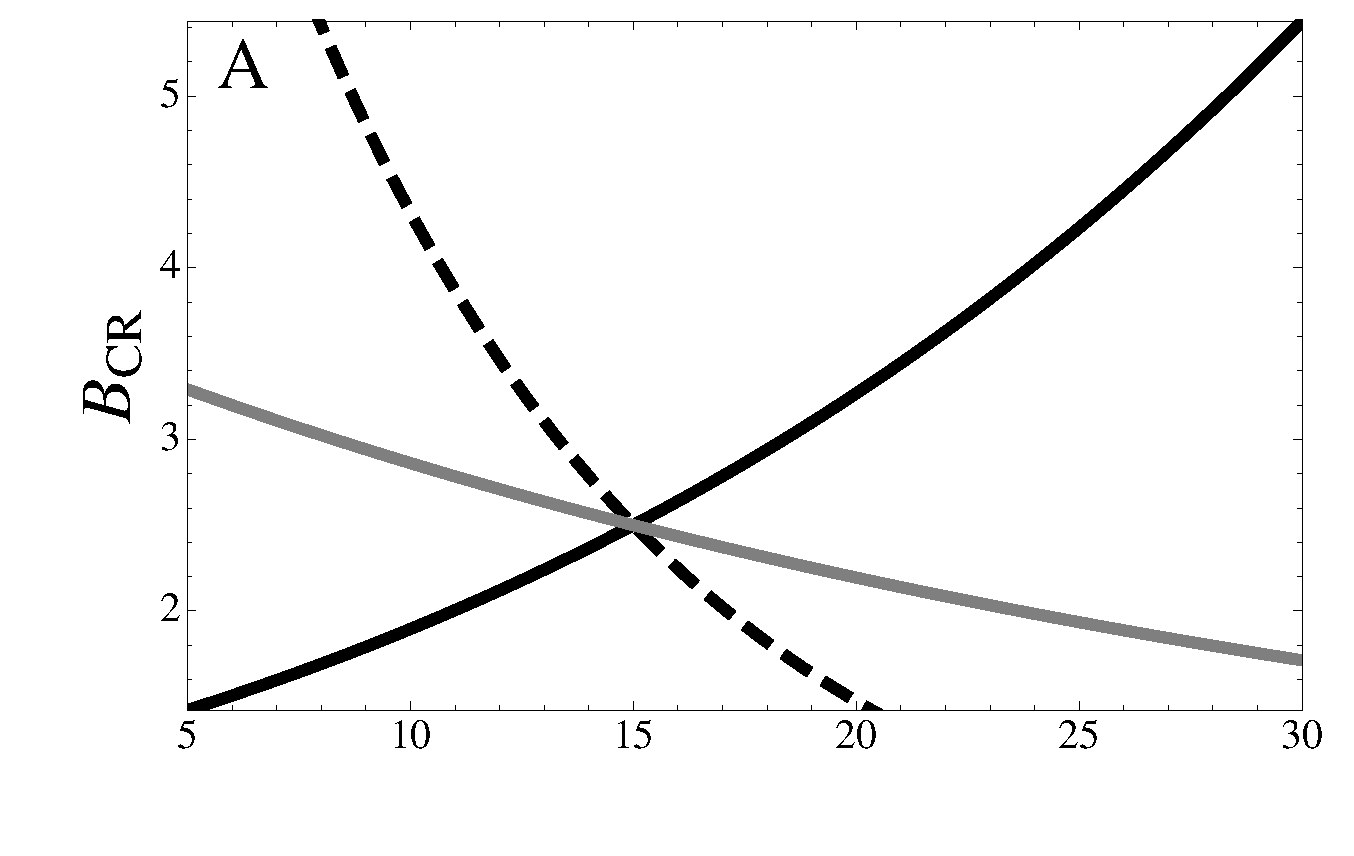
\includegraphics[width=0.5\linewidth]{BCRAllTempDep}
%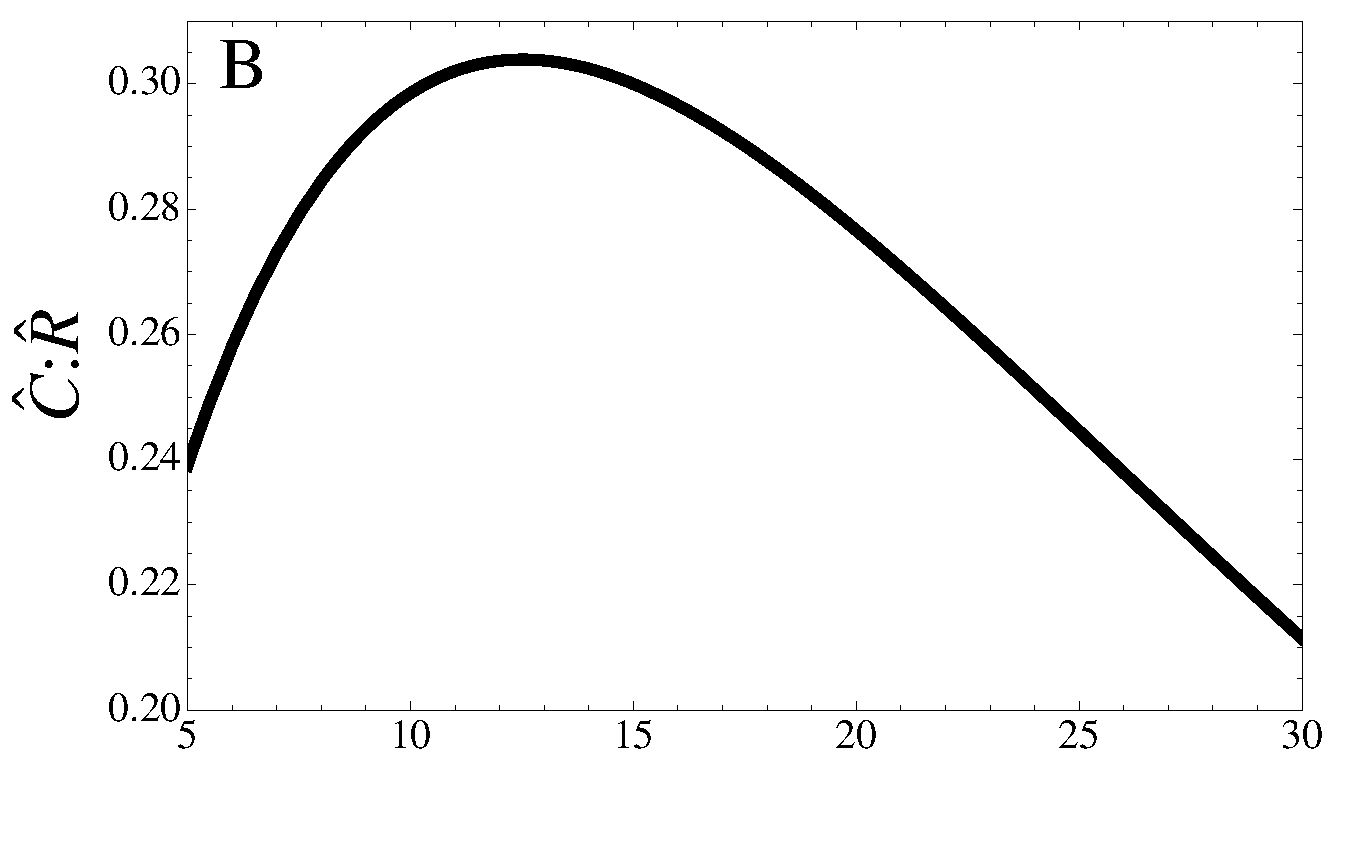
\includegraphics[width=0.5\linewidth]{CtoRAllTempDep}
%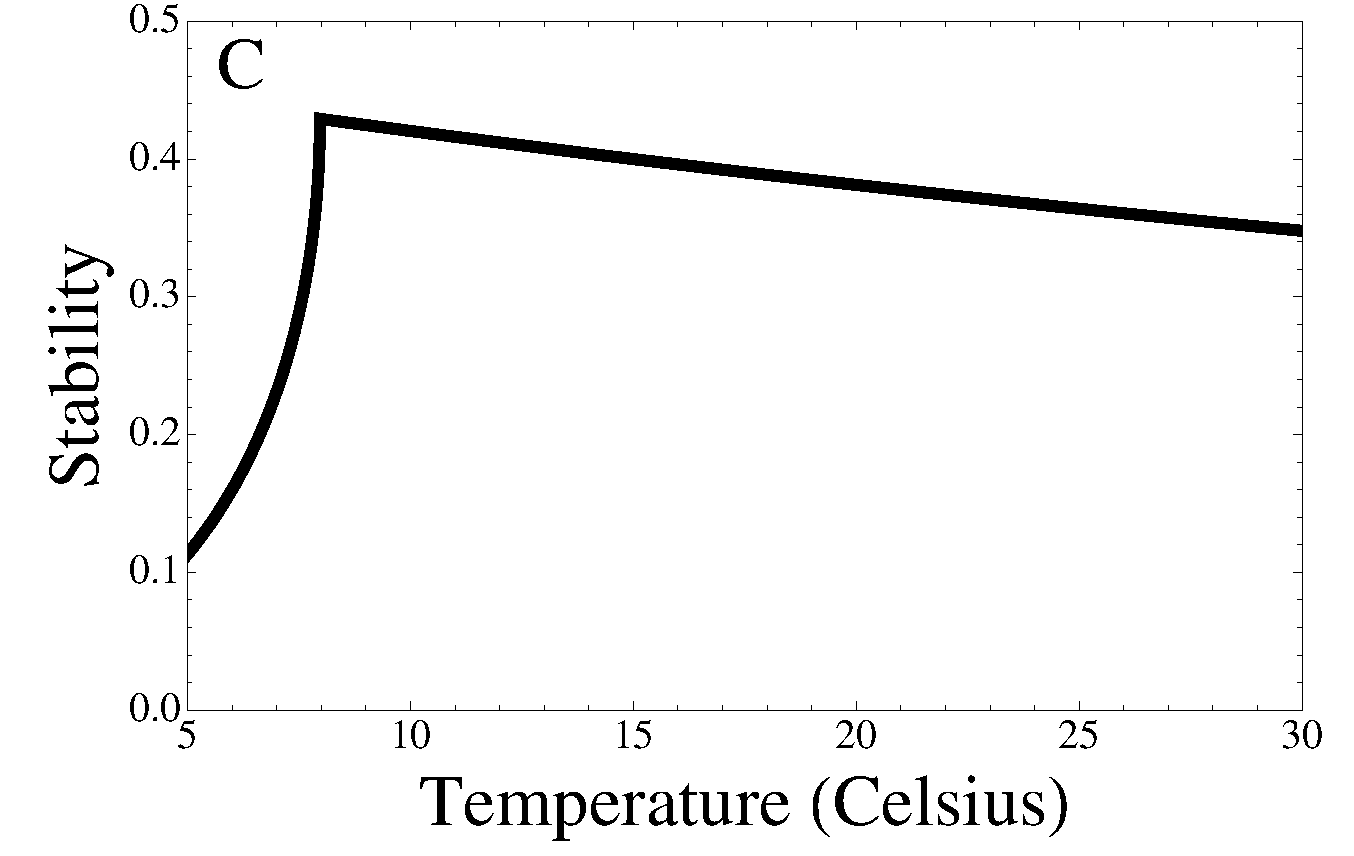
\includegraphics[width=0.5\linewidth]{StabilityAllTempDep}
%\caption{
%$B_{CR}$, equilibrium consumer to resource biomass ratio $\hat{C}:\hat{R}$, and stability of the coexistence equilibrium as functions of temperature $T$ (plotted in Celsius).
%Rate-constants (e.g., $r_0$) were chosen to make $r = 2$, $K = 100$, $a = 0.1$, $m = 0.6$, and $e = 0.15$ at 15$^\circ C$ (as in \cite{Gilbert2014}).
%Other parameters: $E_B = 0.32$ (solid black), $E_B = 0.9$ (dashed and gray), $E_S = 0.9$ (solid black and gray), $E_S = 0.32$ (dashed), $E_m = 0.65$, $E_{\nu,i} = 0.46$, $\nu_{0,i} = 1$.  
%}
%\label{AllTempDep}
%\end{figure}

%%%%%%%%%%%%%%%%%%%%%%%%%%%%%%%%%%%%%%%%%%%%%%%%
\begin{figure}[!ht]
\centering
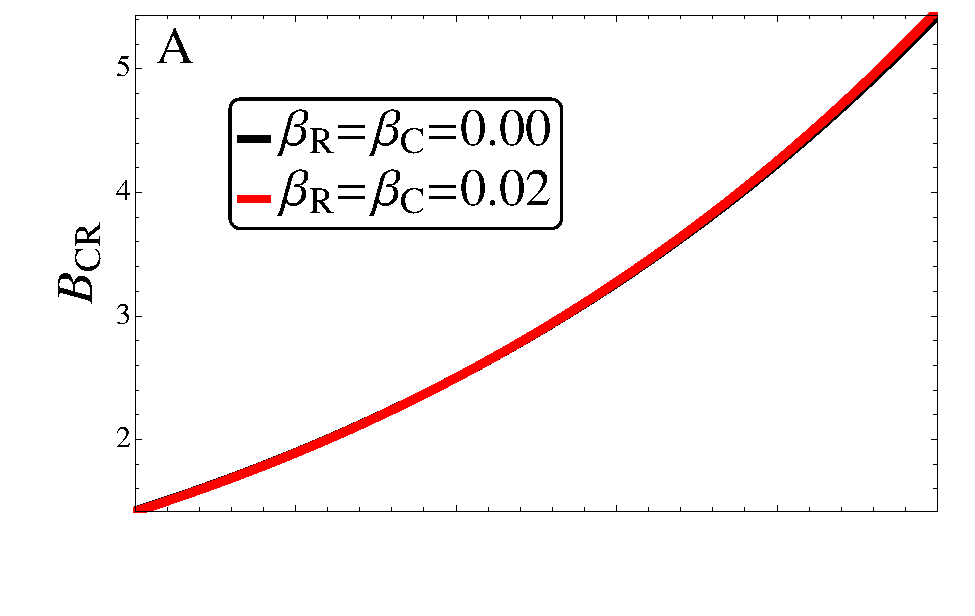
\includegraphics[width=0.5\linewidth]{BCRAllTempMassDep}\\\vspace{-0.75cm}
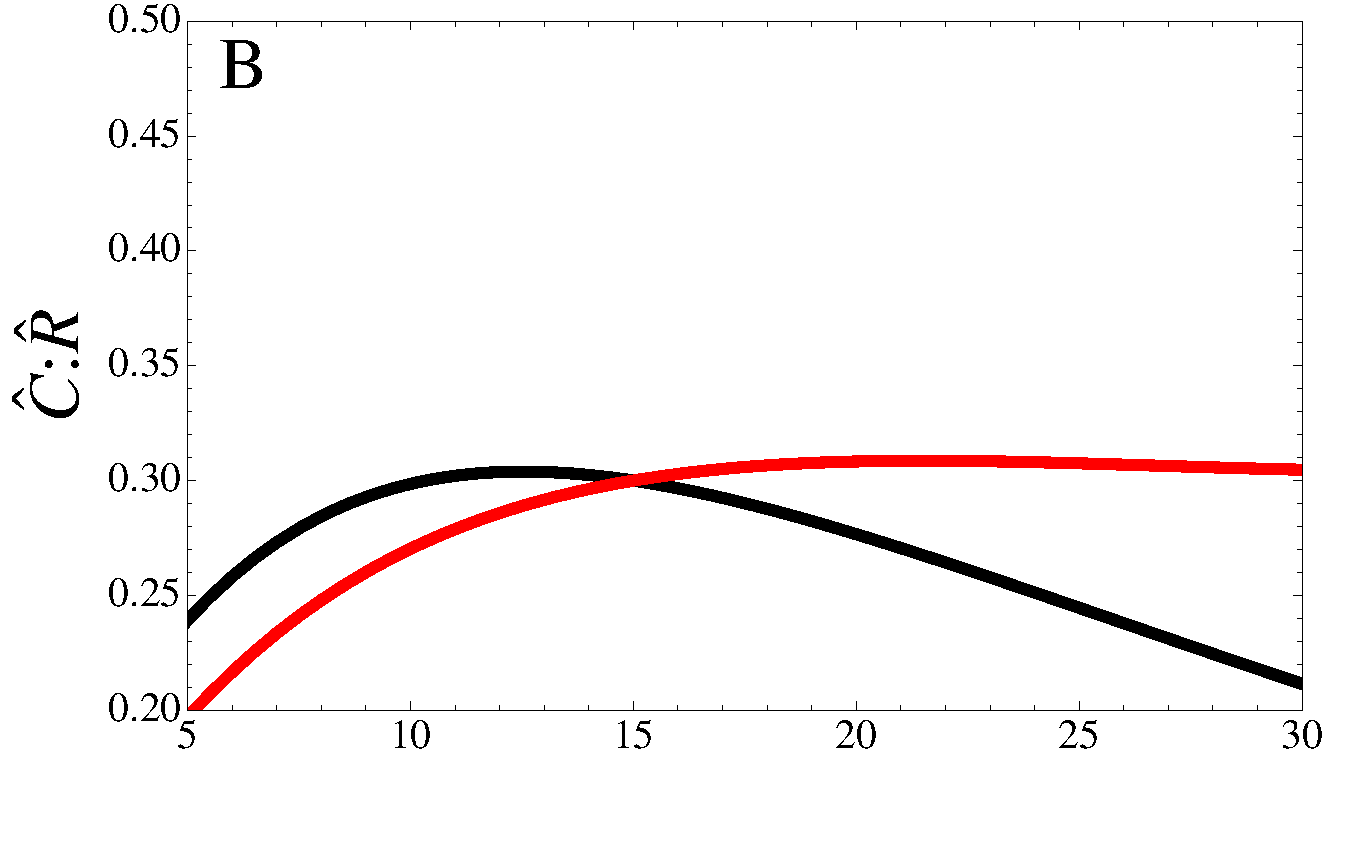
\includegraphics[width=0.5\linewidth]{CtoRAllTempMassDep}\\\vspace{-0.75cm}
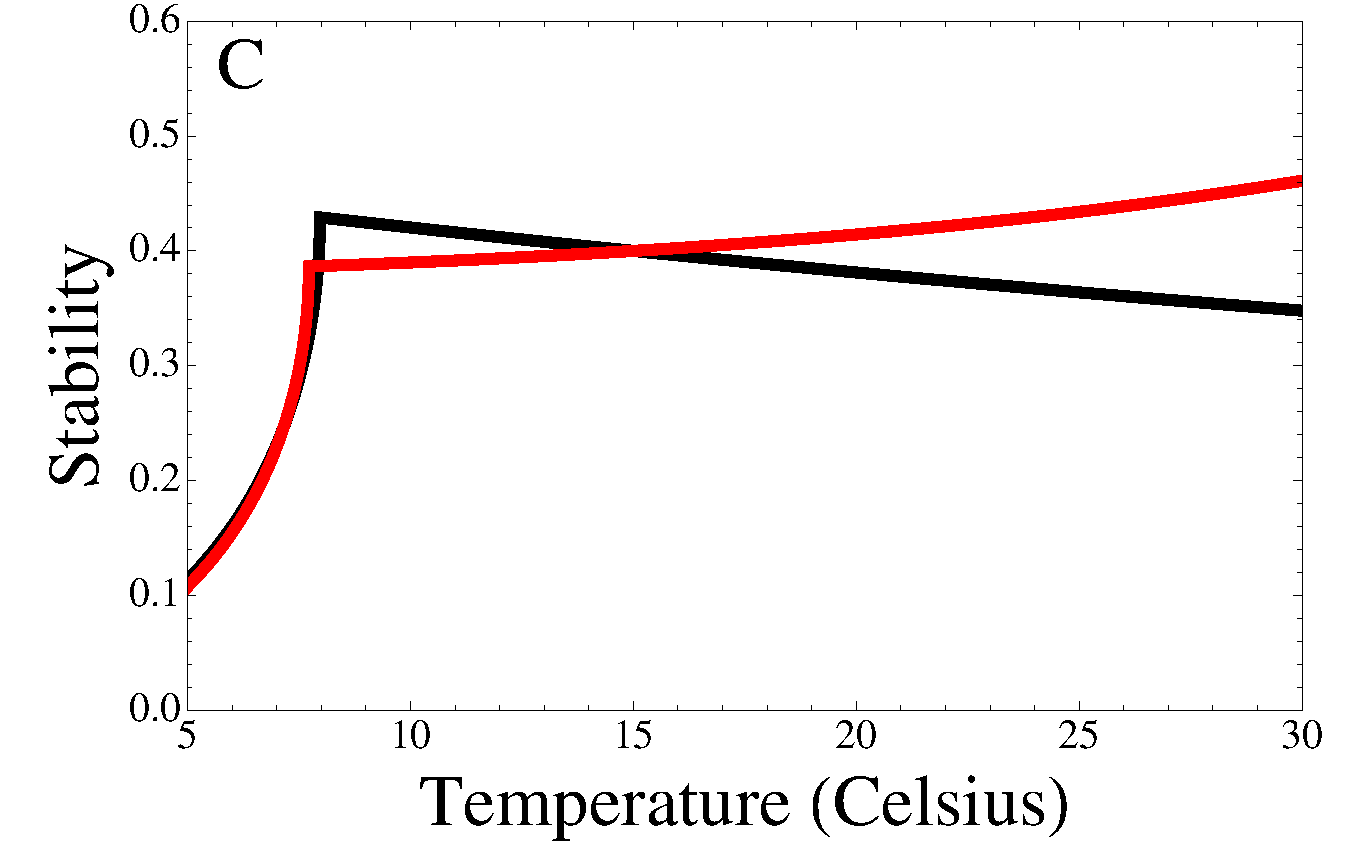
\includegraphics[width=0.5\linewidth]{StabilityAllTempMassDep}
\caption{
$B_{CR}$, equilibrium consumer to resource biomass ratio $\hat{C}:\hat{R}$, and stability of the coexistence equilibrium as functions of temperature $T$ (plotted in Celsius) with (red) and without (black) mass dependencies and the temperature-size rule.
Rate-constants were chosen to make $r = 2$, $K = 100$, $a = 0.1$, $m = 0.6$, and $e = 0.15$ at 15$^\circ C$ \citep[as in Figure 3 of][]{Gilbert2014}.
Other parameters as in \cite{Gilbert2014} and \cite{DeLong2015}: $E_B = 0.32$, $E_S = 0.9$, $E_m = 0.65$, $E_{\nu,i} = 0.46$, $\nu_{0,i} = 1$, $\kappa = -0.81$, $\alpha = 1$, $\epsilon = -0.5$, $\mu = -0.29$, $\rho = -0.81$, $\beta_i = 0$ (black), $\beta_i = 0.02$ (red).  
Note that we allow all population dynamic parameters to depend on temperature and mass, unlike Figure 3 in \cite{Gilbert2014}, where only $K$ varies.
}
\label{AllTempMassDep}
\end{figure}

%%%%%%%%%%%%%%%%%%%%%%%%%%%%%%%%%%%%%%%%%%%%%%%%
\begin{figure}[!ht]
\centering
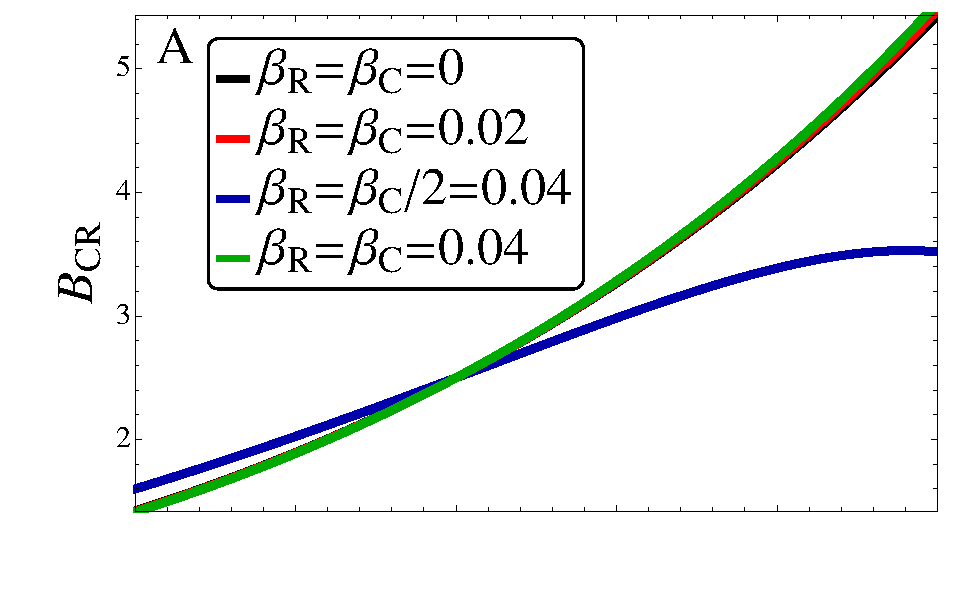
\includegraphics[width=0.5\linewidth]{Figure2A}\\\vspace{-0.75cm}
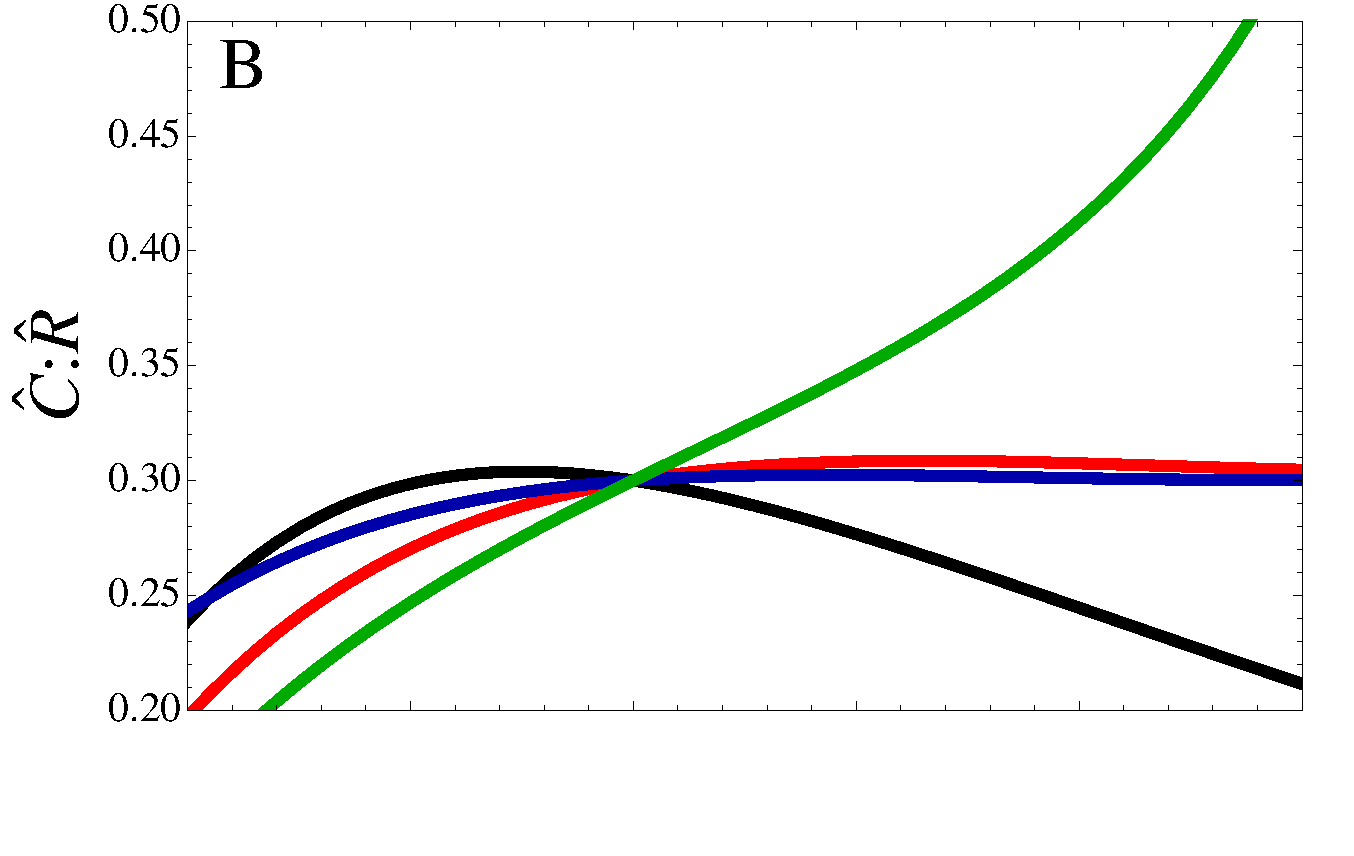
\includegraphics[width=0.5\linewidth]{Figure2B}\\\vspace{-0.75cm}
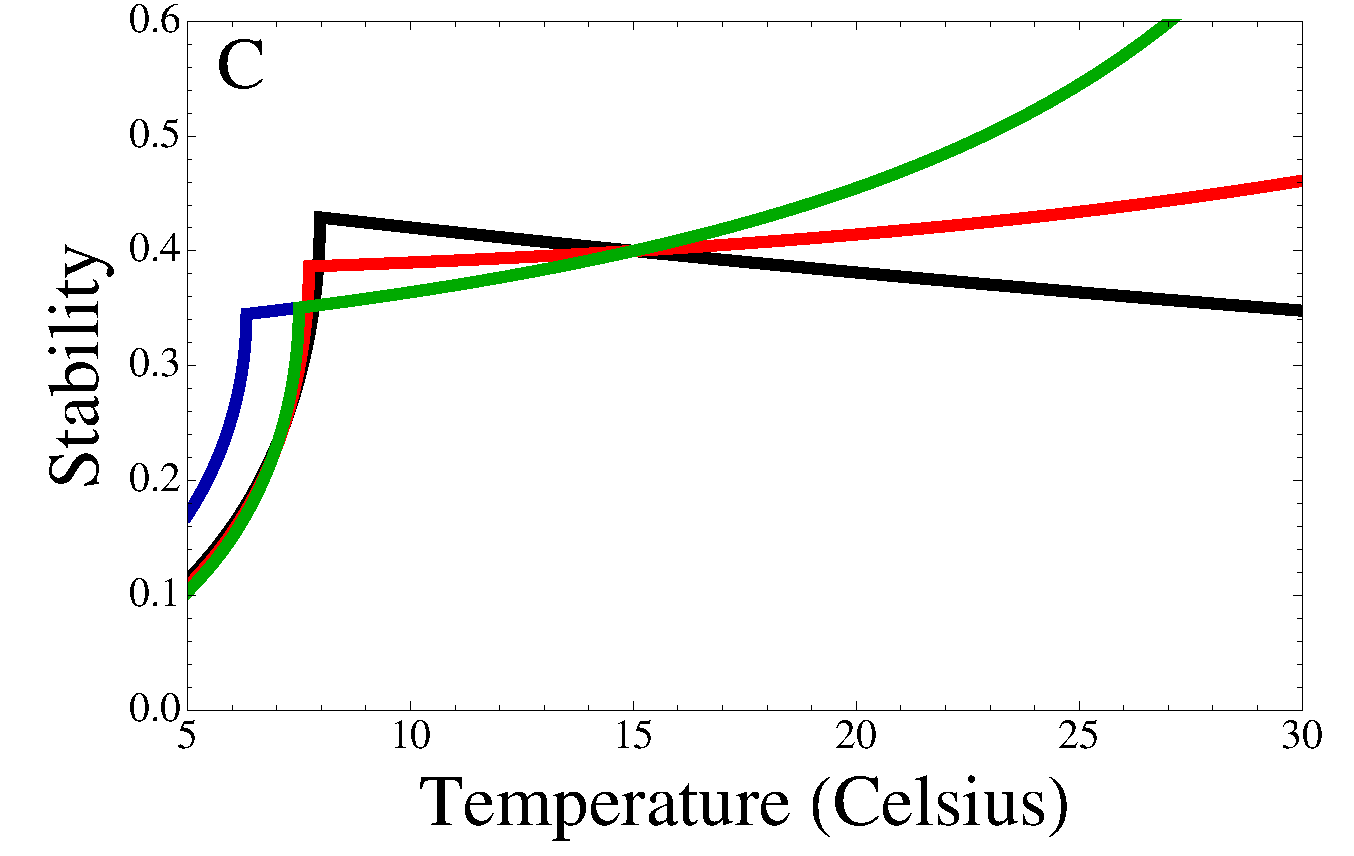
\includegraphics[width=0.5\linewidth]{Figure2C}
\caption{
$B_{CR}$, equilibrium consumer to resource biomass ratio $\hat{C}:\hat{R}$, and stability of the coexistence equilibrium as functions of temperature $T$ (plotted in Celsius) without the temperature-size rule (black), with a relatively weak, symmetric temperature size rule (red), with an asymmetric temperature-size rule (green), and with a relatively strong, symmetric temperature-size rule (blue).
Rate-constants were chosen to make $r = 2$, $K = 100$, $a = 0.1$, $m = 0.6$, and $e = 0.15$ at 15$^\circ C$ \citep[as in Figure 3 of][]{Gilbert2014}.
Other parameters as in \cite{Gilbert2014} and \cite{DeLong2015}: $E_B = 0.32$, $E_S = 0.9$, $E_m = 0.65$, $E_{\nu,i} = 0.46$, $\nu_{0,i} = 1$, $\kappa = -0.81$, $\alpha = 1$, $\epsilon = -0.5$, $\mu = -0.29$, $\rho = -0.81$.
}
\label{StrengthAsymm}
\end{figure}

%%%%%%%%%%%%%%%%%%%%%%%%%%%%%%%%%%%%%%%%%%%%%%%%
\begin{figure}[!ht]
\centering
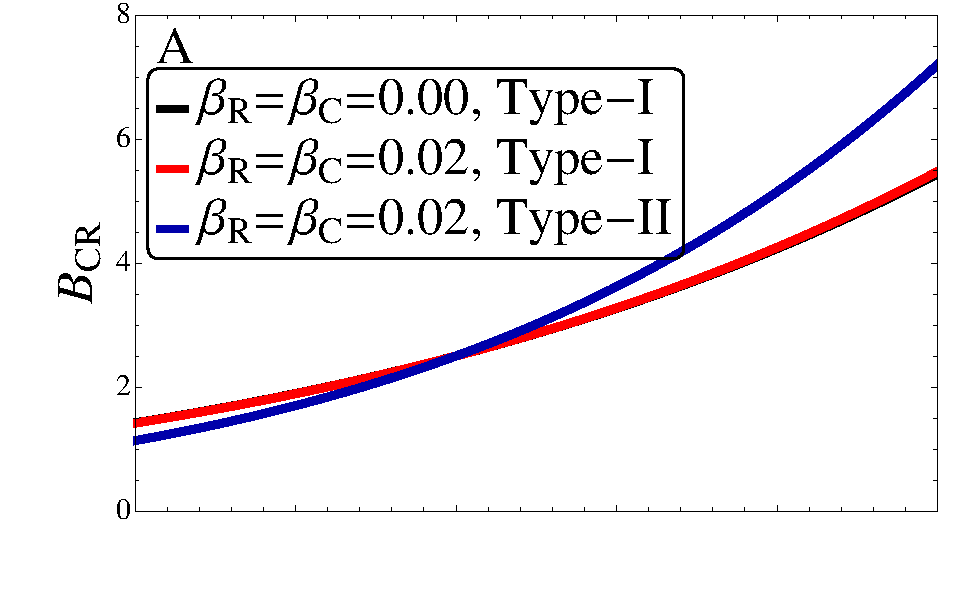
\includegraphics[width=0.5\linewidth]{BCRTypeII}\\\vspace{-0.75cm}
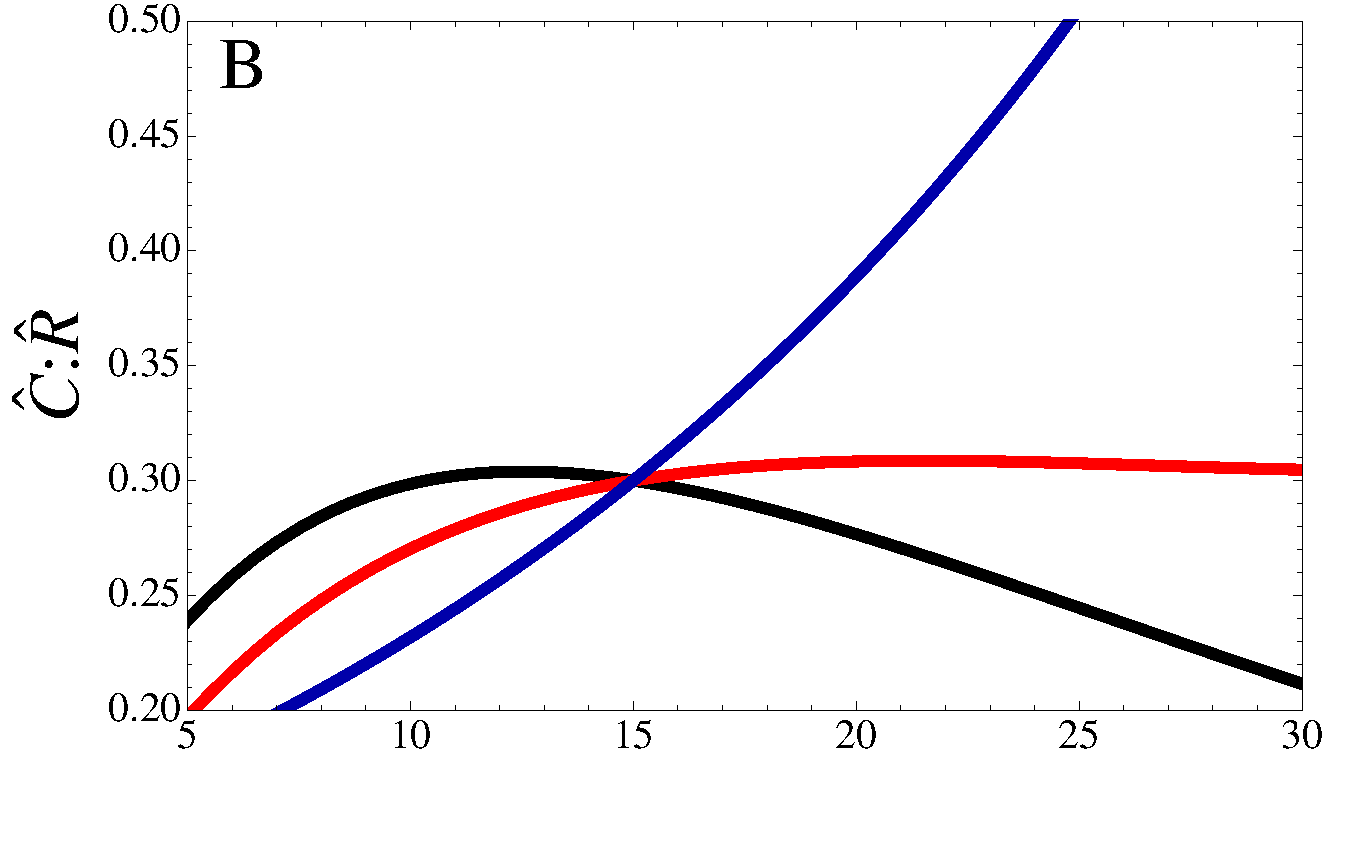
\includegraphics[width=0.5\linewidth]{CtoRTypeII}\\\vspace{-0.75cm}
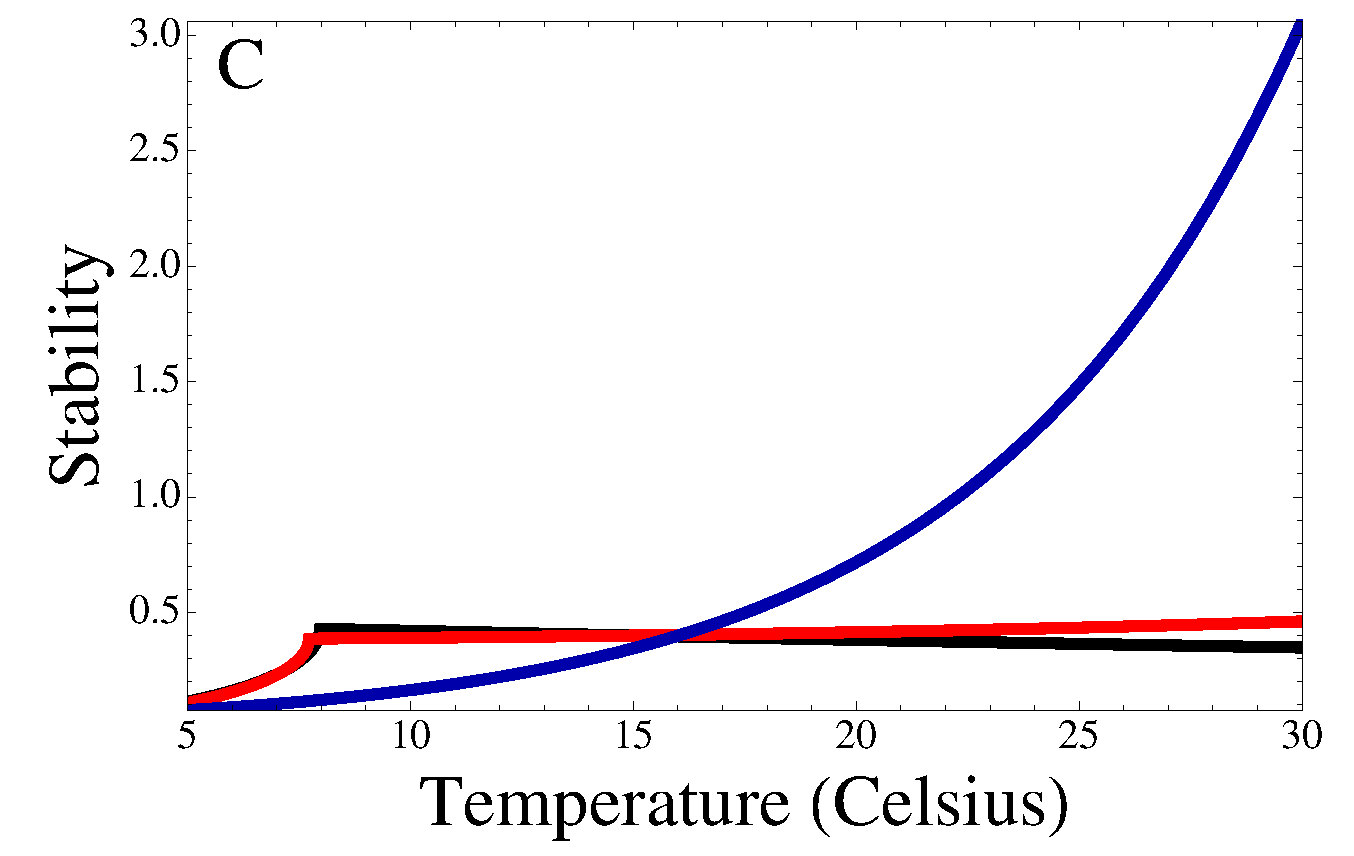
\includegraphics[width=0.5\linewidth]{StabilityTypeII}
\caption{
$B_{CR}$, equilibrium consumer to resource biomass ratio $\hat{C}:\hat{R}$, and stability of the coexistence equilibrium as functions of temperature $T$ (plotted in Celsius) with (red and blue) and without (black) mass dependencies and the temperature-size rule.
Type-II functional response in blue.
Rate-constants were chosen to make $r = 2$, $K = 100$, $f(R) = 0.1$, $m = 0.6$, and $e = 0.15$ at 15$^\circ C$ (as in Figure 3 of \cite{Gilbert2014}).
Other parameters as in \cite{Gilbert2014}, \cite{DeLong2015}, and \cite{Rall2012}: $E_B = 0.32$, $E_S = 0.9$, $E_m = 0.65$, $E_{\nu,i} = 0.46$, $\nu_{0,i} = 1$, $\kappa = -0.81$, $\alpha = 1$, $\epsilon = -0.5$, $\mu = -0.29$, $\rho = -0.81$, $a_C = 1/4+2/3$, $a_R = 1/3$, $h_C = -2/3$, $h_R = 0.5$, $E_a = 0.65$, $E_h = -0.65$, $h_0 = 10^{-13}$.  
}
\label{TypeII}
\end{figure}

%%%%%%%%%%%%%%%%%%%%%%%%%%%%%%%%%%%%%%%%%%%%%%%%
%\begin{figure}[!ht]
%\centering
%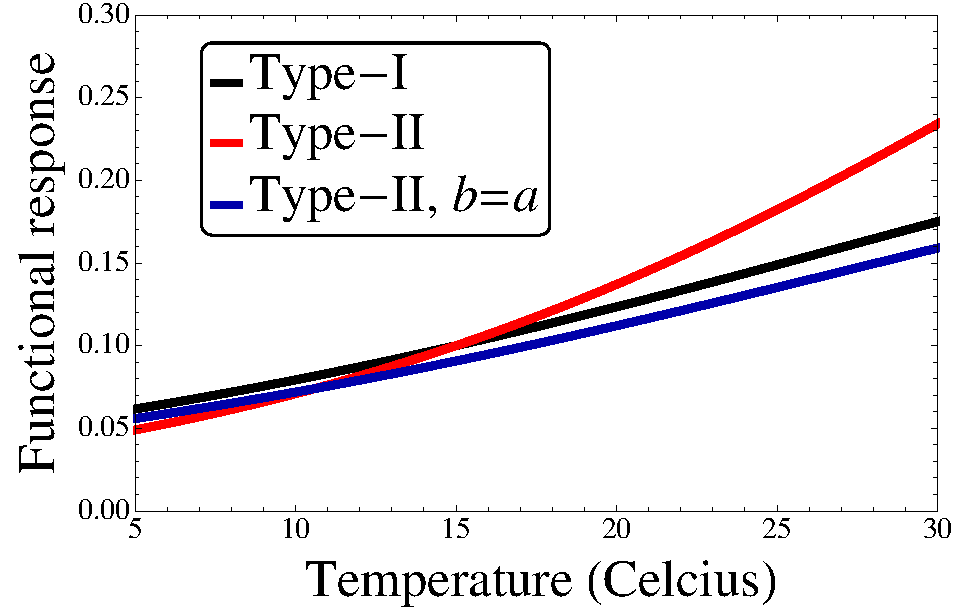
\includegraphics[width=0.5\linewidth]{FunctionalResponseTemp}
%\caption{
%SUPPLEMENTARY FIGURE. Functional response as a function of temperature.
%Shown are a type-I functional response (black), a type-II functional response with temperature- and mass-dependencies of capture rate and handling time from \cite{Rall2012} (red), and a type-II functional response with temperature- and mass-dependencies of capture rate like that of attack rate in \cite{Gilbert2014} (blue).
%Rate-constants were chosen to make $r = 2$, $K = 100$, $a = 0.1$, $m = 0.6$, and $e = 0.15$ at 15$^\circ C$ \citep[as in Figure 3 of][] {Gilbert2014}.
%Other parameters as in \cite{Gilbert2014}, \cite{DeLong2015}, and \cite{Rall2012}: $E_B = 0.32$, $E_S = 0.9$, $E_m = 0.65$, $E_{\nu,i} = 0.46$, $\nu_{0,i} = 1$, $\kappa = -0.81$, $\alpha = 1$, $\epsilon = -0.5$, $\mu = -0.29$, $\rho = -0.81$, $\beta_i = 0.02$, $a_C = 1/4+2/3$, $a_R = 1/3$, $h_C = -2/3$, $h_R = 0.5$, $E_a = 0.65$, $E_h = -0.65$, $h_0 = 10^{-13}$.  
%}
%\label{FunctionalResponseTemp}
%\end{figure}

%%%%%%%%%%%%%%%%%%%%%%%%%%%%%%%%%%%%%%%%%%%%%%%%
%\begin{figure}[!ht]
%\centering
%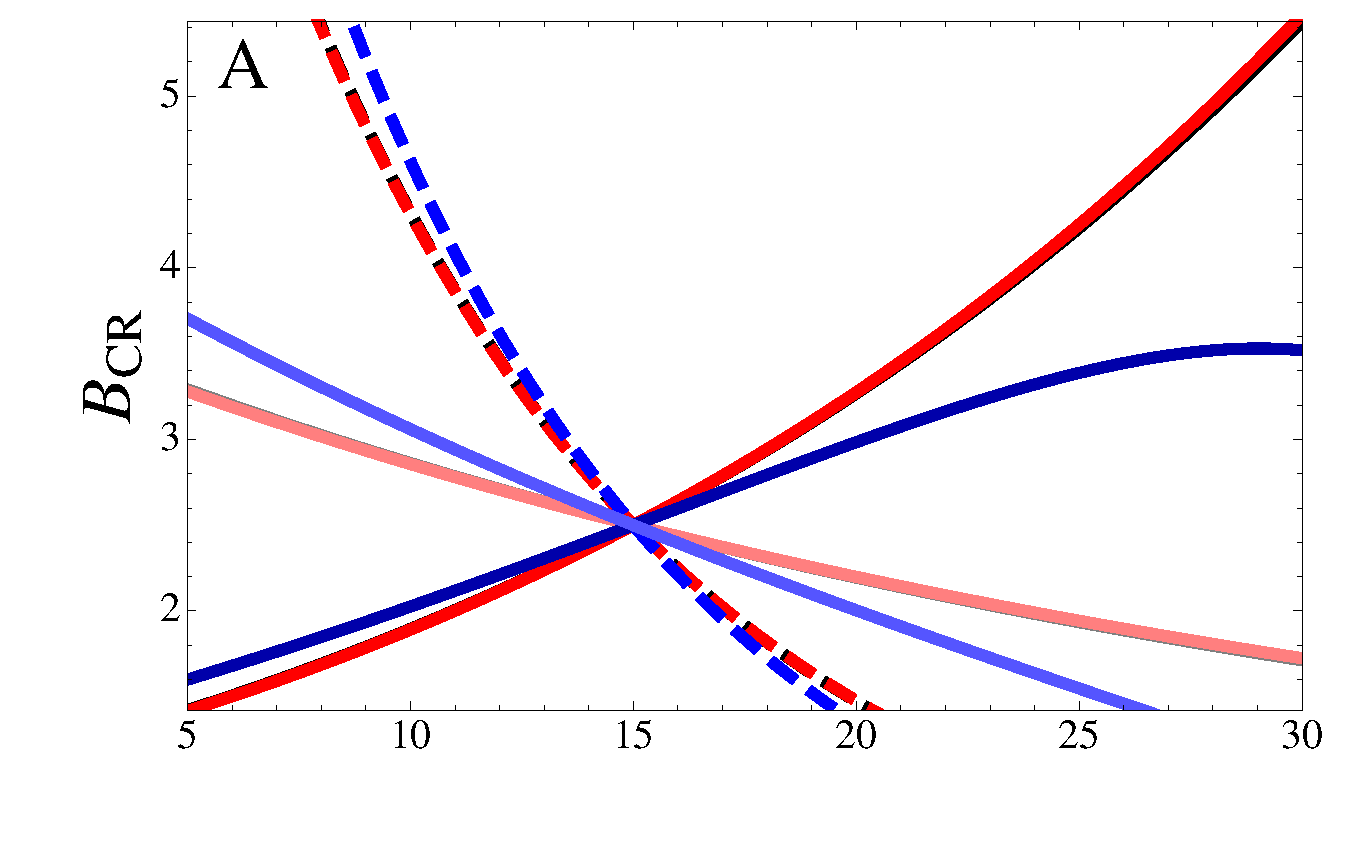
\includegraphics[width=0.5\linewidth]{BCRAllTempMassDepAsymm}\\\vspace{-0.75cm}
%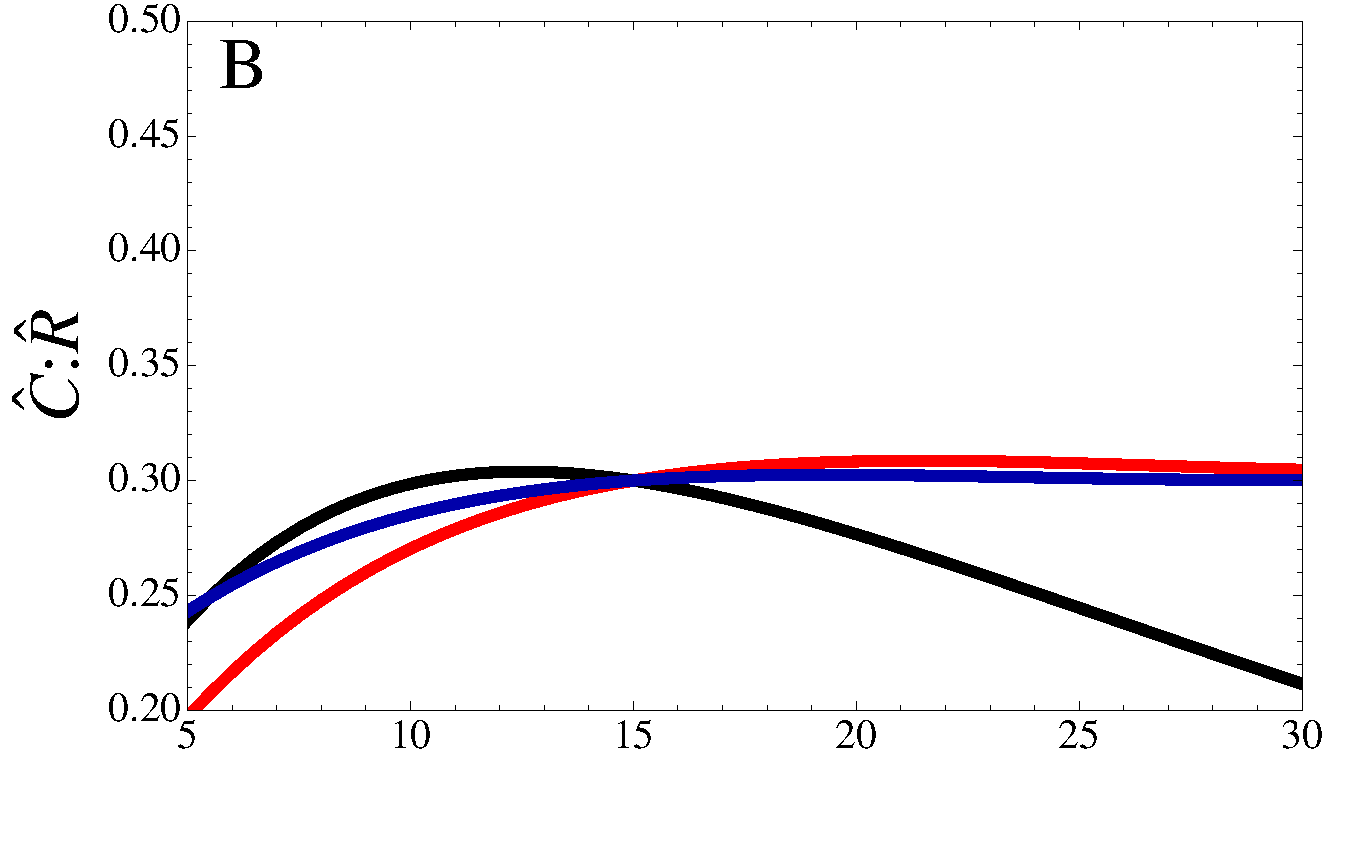
\includegraphics[width=0.5\linewidth]{CtoRAllTempMassDepAsymm}\\\vspace{-0.75cm}
%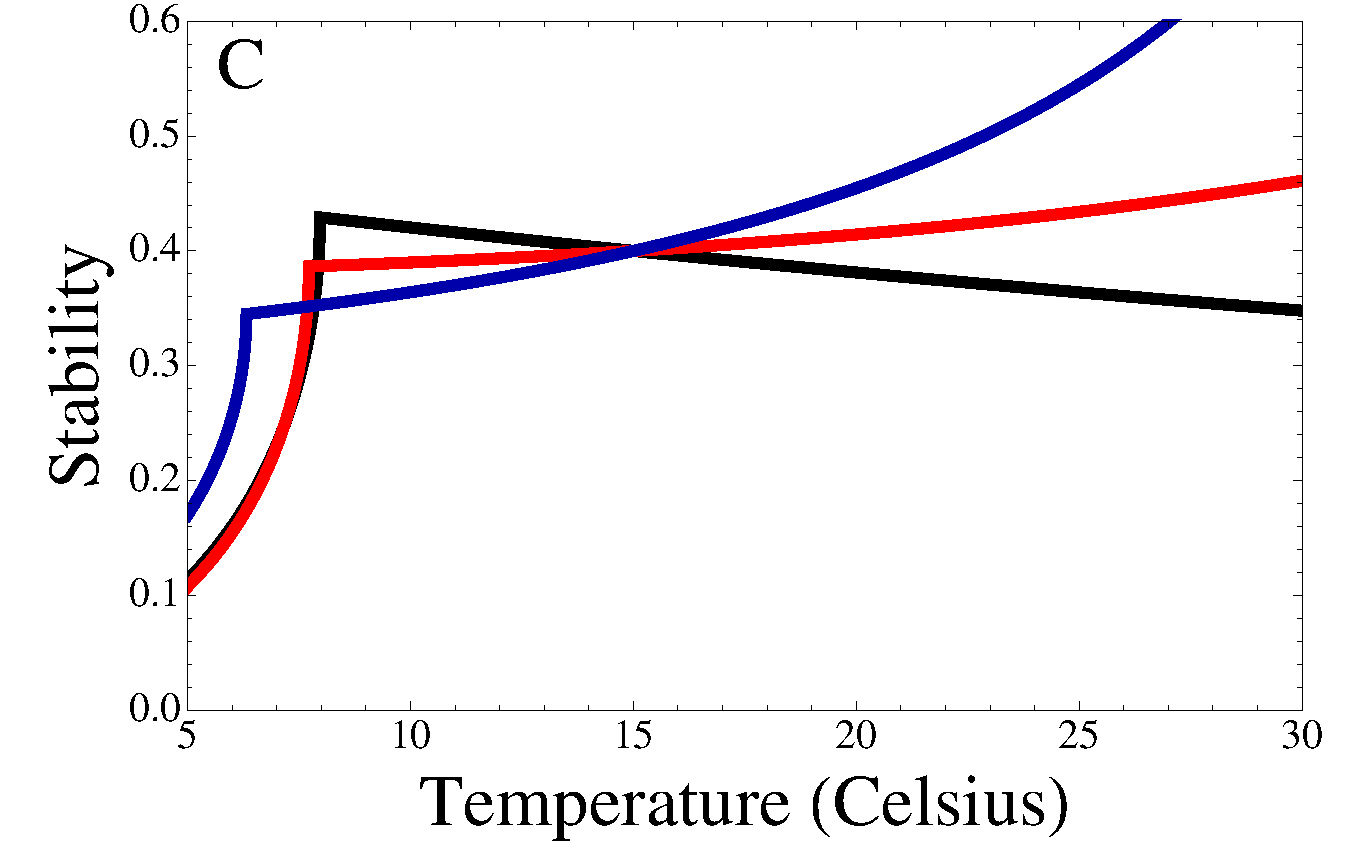
\includegraphics[width=0.5\linewidth]{StabilityAllTempMassDepAsymm}
%\caption{
%SUPPLEMENTARY FIGURE.
%$B_{CR}$, equilibrium consumer to resource biomass ratio $\hat{C}:\hat{R}$, and stability of the coexistence equilibrium as functions of temperature $T$ (plotted in Celsius) without the temperature-size rule (black) with a symmetric temperature-size rule (red) and with an asymmetric temperature-size rule (blue).
%Rate-constants (e.g., $r_0$) were chosen to make $r = 2$, $K = 100$, $a = 0.1$, $m = 0.6$, and $e = 0.15$ at 15$^\circ C$ (as in \cite{Gilbert2014}).
%Other parameters as in \cite{Gilbert2014,DeLong2015,Forster2012}: $E_B = 0.32$ (solid dark), $E_B = 0.9$ (dashed and solid light), $E_S = 0.9$ (solid), $E_S = 0.32$ (dashed), $E_m = 0.65$, $E_{\nu,i} = 0.46$, $\nu_{0,i} = 1$, $\kappa = -0.81$, $\alpha = 1$, $\epsilon = -0.5$, $\mu = -0.29$, $\rho = -0.81$, $\beta_i = 0$ (black) , $\beta_i = 0.02$ (red), $\beta_R = 0.02$ and $\beta_C = 0.04$ (blue).  
%}
%\label{AllTempMassDepAsymm}
%\end{figure}

%%%%%%%%%%%%%%%%%%%%%%%%%%%%%%%%%%%%%%%%%%%%%%%%
%\begin{figure}[!ht]
%\centering
%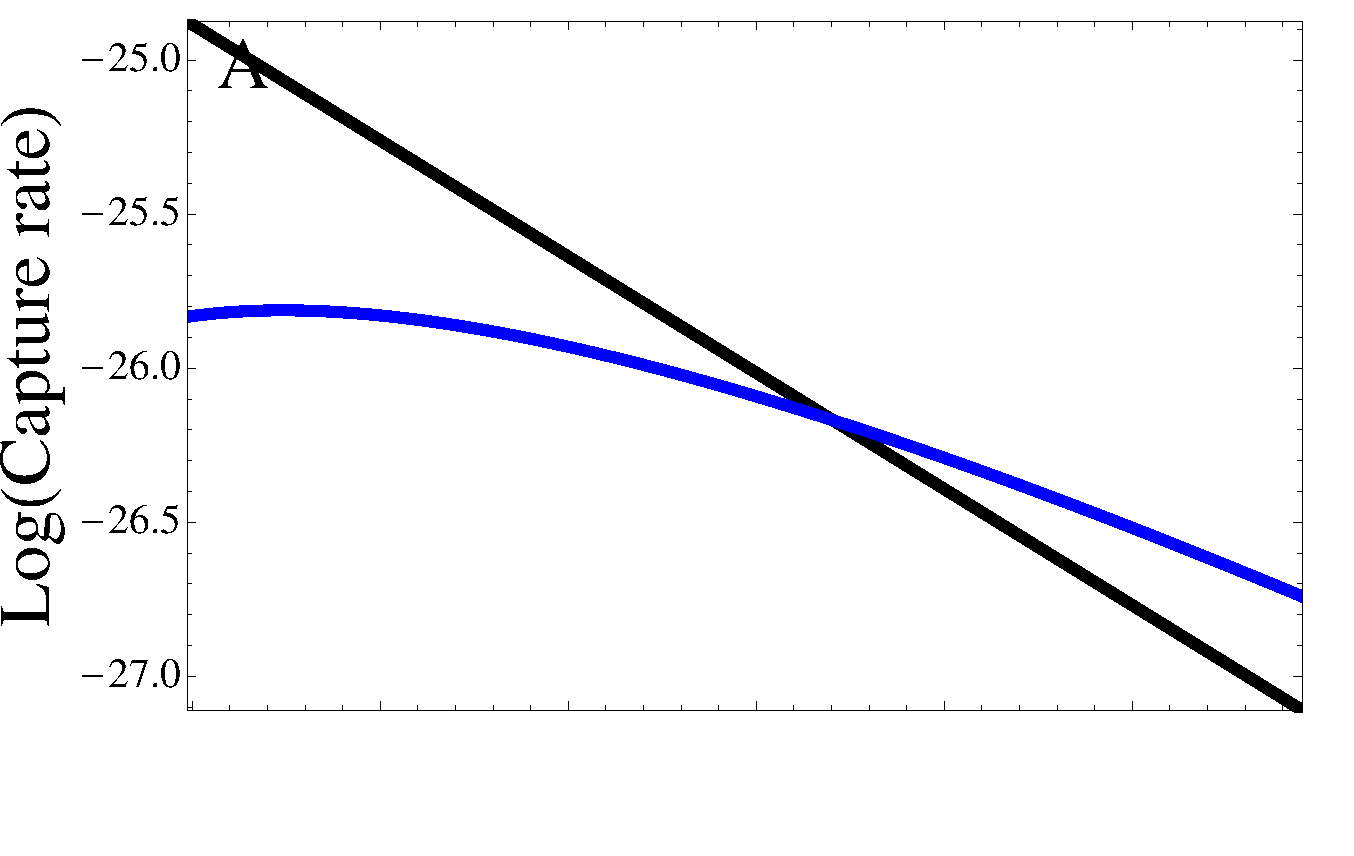
\includegraphics[width=0.5\linewidth]{CaptureTSRAsymm}\\\vspace{-0.75cm}
%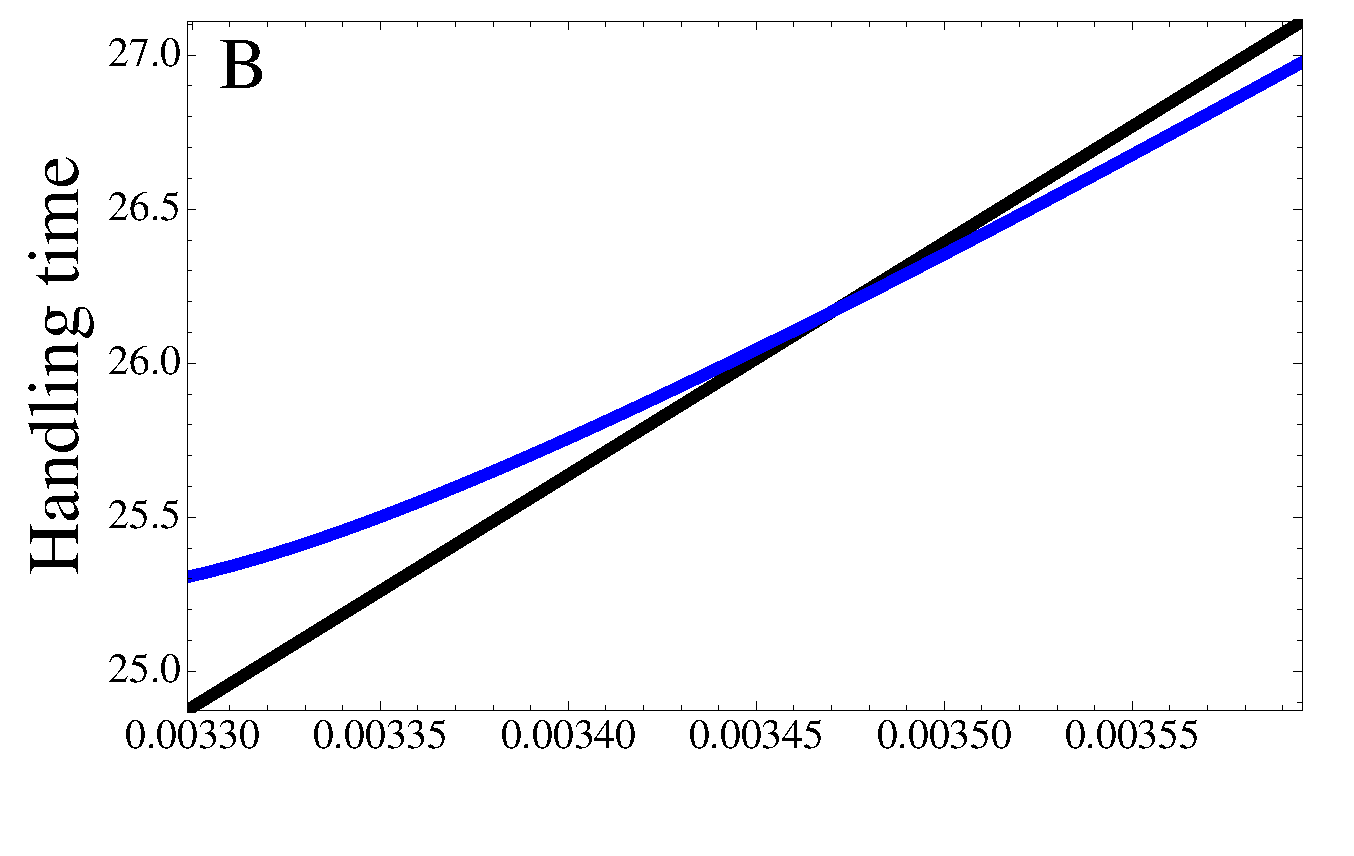
\includegraphics[width=0.5\linewidth]{HandlingTSRAsymm}
%\caption{
%SUPPLEMENTARY FIGURE.
%The sensitivity of capture rate and handling time to temperature with (blue) and without (black) the temperature-size rule.
%Plotted are (A) $\log(b/b0)$ and (B) $\log(h/h0)$.
%Parameters as in \cite{Rall2012}: $a_C = 1/4+2/3$, $a_R = 1/3$, $h_C = -2/3$, $h_R = 0.5$, $E_a = 0.65$, $E_h = -0.65$.
%}
%\label{CaptureTimeT}
%\end{figure}

\end{document}
